%Question 3

\begin{enumerate}
	
	%Part a
	\item{
		Design $2^{nd}$ order filter by cascading two first order filters together, followed by a gain stage.\\
		\\
		Design the filter by starting with prototype stages then frequency and magnitude scaling to get desired properties. \\
		\\
		Now a prototype first order active high pass filter has unity gain in the passband and a cutoff frequency of $\omega_c = 1$ rad/s, and is of form:
		\begin{figure}[H]
			\centering
			\begin{circuitikz}
				\draw (0,2.5) to[short] (0.5,2.5)
					to[R=$1 \, \Omega$] (2.5,2.5)	% cannot use = on own in label, must escape with {=} then manage spacing
					to[C=$1 \, \text{F}$] (4,2.5)
					to[short] (4,4) 
					to[R=$1 \, \Omega$] (7,4)
					to[short] (7,2);
				\draw (0,2.5) to[open, v_=$v_i$, o-o] (0,0);
				\draw (0,0) to[short, o-o] (8,0);
				\draw (5.5,2) node[op amp] (opamp) {}
					(opamp.-) to[short, -*] (4,2.5) 
					(opamp.+) to[short] (4,1.5) to[short,-*] (4,0)
					(opamp.out) to[short, -*] (7,2) to[short, -o] (8,2);
				\draw(8,0) to [open, v<=$v_o$, o-o] (8,2);
			\end{circuitikz}
		\end{figure}
		Noting that a circuit of this form has transfer function:
		\begin{equation*}
			H_L(s) = \frac{-s}{s+1}
		\end{equation*}
		Now when two of these are connected in cascade, the overall transfer function is:
		\begin{align*}
			H(s) &= H_L(s) \cdot H_L(s) \\
			&= \frac{s^2}{(s+1)^2}
		\end{align*}
		We know this transfer function describes a 2$^{\text{nd}}$ order high pass filter with a passband gain of 1 V/V. Now find the cutoff frequency:
		\begin{equation*}
			\omega_c \triangleq \omega : \big|H(j\omega)\big| = \frac{1}{\sqrt{2}}
		\end{equation*}
		So first find $|H(j\omega)|$:
		\begin{align*}
			H(j\omega) &= H(s)\big{|}_{s = j\omega} \\
			&= \frac{(j\omega)^2}{(j\omega+1)^2} \\
			&= \frac{-\omega^2}{(j\omega+1)^2} \\
			\\
			\big|H(j\omega)\big| &= \frac{\big|-\omega^2\big|}{\big|j\omega+1\big|^2} \\
			&= \frac{\omega^2}{\Big(\sqrt{\omega^2+1^2}\Big)^2} \\
			&= \frac{\omega^2}{\omega^2+1}
		\end{align*}
		Now find $\omega_c$:
		\begin{align*}
			\big|H(j\omega_c)\big| &= \frac{1}{\, \sqrt{2 \,} \,} \\
			\therefore \frac{\omega_c^2}{\, \omega_c^2+1 \,} &= \frac{1}{\, \sqrt{2 \,} \,} \\
			\therefore \sqrt{2 \,} \cdot \omega_c^2 - \omega_c^2 &= 1 \\
			\therefore \omega_c^2 &= \frac{1}{\, \sqrt{2 \,} - 1 \,} \\
			\therefore \omega_c &= \frac{1}{\, \sqrt{\sqrt{2 \,} - 1 \,} \,} \\
			&= 1.554 \ \text{rad/s}
		\end{align*}
		Noting that the negative root of $\omega_c$ has been rejected, as we define $\omega \geq 0$ rad/s. \\
		We now know this prototype 2$^{\text{nd}}$ order active high pass filter has a passband gain of 1 V/V and a cutoff frequency of 1.554 rad/s. \\ 
		\\
		Now we need to modify this prototype design to match the parameters we want. We do this by frequency scaling and magnitude scaling the response, and hence the circuit. \\
		\\
		First we will frequency scale to the desired cutoff frequency of 1 kHz. We do this by finding the frequency scaling factor $k_f \triangleq \frac{\omega_c^{'}}{\omega_c}$, where $\omega_c^{'}$ is the desired cutoff frequency and $\omega_c$ is the current cutoff frequency:
		\begin{align*}
			k_f &= \frac{2 \cdot \pi \cdot 1000}{1.554} \\
			&= 4043.8
		\end{align*}
		Now we note that we must use 100 nF capacitors in the final design. Therefore we find the magnitude scaling factor from the following equation:
		\begin{equation*}
			k_m = \frac{C}{C^{'} \cdot k_f}
		\end{equation*}
		Where C is the prototypical circuit's capacitor value and $C^{'}$ is the desired capacitor value:
		\begin{align*}
			k_m &= \frac{1}{100 \times 10^{-9} \cdot 4043.8} \\
			&= 2472.9
		\end{align*}
		Now scale the resistor from the prototypical value ($R$) to the desired value ($R^{'}$):
		\begin{align*}
			R^{'} &= k_m \cdot R \\
			&= 2472.9 \cdot 1 \\
			&= 2.47 \ \text{k}\Omega
		\end{align*}
		Now we want a gain of 1 V/V in the passband in these filter stages, so we want $R_s^{'} = R_f^{'} = 2.47 \ \text{k}\Omega$. \\
		\\
		Now we need to design the gain stage, achieve this using an op amp in the inverting amplifier configuration:
		\begin{figure}[H]
			\centering
			\begin{circuitikz}
				\draw (0,2.5) to[open, v=$v_i$] (0,0) 
					to [short, o-o] (7,0);
				\draw (0,2.5) to [short, o-] (0.5,2.5)
					to [R=$R_s$] (2.5,2.5)
					to [short] (3,2.5)
					to [short] (3,4)
					to [R=$R_f$] (6,4)
					to [short] (6,2);
				\draw (4.5,2) node[op amp] (opamp) {}
					(opamp.-) to [short, -*] (3,2.5)
					(opamp.+) to [short] (3,1.5)
						to [short, -*] (3,0)
					(opamp.out) to [short, -*] (6,2)
						to [short, -o] (7,2);
				\draw (7,0) to [open, v<=$v_o$] (7,2);
			\end{circuitikz}
		\end{figure}
		We know this circuit has transfer function $H(s) = -\frac{R_f}{R_s}$\\
		Now we want a passband gain of 10 V/V. Therefore in the gain stage we want:
		\begin{align*} 
			\big|H(s)\big| &= 10 \\
			\therefore \frac{R_f}{R_s} &= 10, \qquad \text{let $R_s$ = 1 k$\Omega$,} \implies R_f = 10 \ \text{k}\Omega
		\end{align*}
		Therefore the overall design is:
		\begin{figure}[H]
			\centering
			\scalebox{0.625}{
				\begin{circuitikz}
					\draw (0,2.5) to [short] (0.5,2.5)
						to [R=$2.47 \, \text{k}\Omega$] (2.5,2.5)
						to [C=$100 \, \text{nF}$] (4,2.5)
						to [short] (4,4) 
						to [R=$2.47 \, \text{k}\Omega$] (7,4)
						to [short] (7,2);
					\draw (0,2.5) to [open, v_=$v_i$, o-o] (0,0);
					\draw (0,0) to [short, o-o] (24,0);
					\draw (5.5,2) node[op amp] (opamp) {}
						(opamp.-) to [short, -*] (4,2.5) 
						(opamp.+) to [short] (4,1.5) to[short,-*] (4,0)
						(opamp.out) to [short, -*] (7,2) to[short] (8,2);

					\draw (8,2) to [short] (8,2.5)
						to [short] (8.5,2.5)
						to[R=$2.47 \, \text{k}\Omega$] (10.5,2.5)
						to[C=$100 \, \text{nF}$] (12.5,2.5)
						to[short] (12.5,4) 
						to[R=$2.47 \, \text{k}\Omega$] (15.5,4)
						to[short] (15.5,2);
					\draw (14,2) node[op amp] (opamp) {}
						(opamp.-) to[short, -*] (12.5,2.5) 
						(opamp.+) to[short] (12.5,1.5) to[short,-*] (12.5,0)
						(opamp.out) to[short, -*] (15.5,2) to[short] (16.5,2);

					\draw (16.5,2) to [short] (16.5,2.5)
						to [short] (17,2.5)
						to [R=$1 \, \text{k}\Omega$] (19,2.5)
						to [short] (19.5,2.5)
						to [short] (19.5,4)
						to [R=$10 \, \text{k}\Omega$] (22.5,4)
						to [short] (22.5,2);
					\draw (21,2) node[op amp] (opamp) {}
						(opamp.-) to [short, -*] (19.5,2.5)
						(opamp.+) to [short] (19.5,1.5)
							to [short, -*] (19.5,0)
						(opamp.out) to [short, -*] (22.5,2)
							to [short, -o] (24,2);
					\draw (24,0) to [open, v<=$v_o$] (24,2);
				\end{circuitikz}
			}
		\end{figure}
	}
	
	%Part b
	\item{
		Re-draw circuit in s domain:
		\begin{figure}[H]
			\centering
			\scalebox{0.625}{
				\begin{circuitikz}
					\draw (0,2.5) to [short] (0.5,2.5)
						to [R=$2.47 \, \text{k}\Omega$] (2,2.5)
						to [C=$\frac{10^7}{s} \, \Omega$, i_=$I_{s1}(s)$] (4.5,2.5)
						to [short] (4.5,4) 
						to [R=$2.47 \, \text{k}\Omega$, i_=$I_a(s)$] (7.5,4)
						to [short] (7.5,2);
					\draw (0,2.5) to [open, v_=$V_i(s)$, o-o] (0,0);
					\draw (0,0) to [short, o-o] (23.5,0);
					\draw (6,2) node[op amp] (opamp) {}
						(opamp.-) to [short, -*] (4.5,2.5) 
						(opamp.+) to [short] (4.5,1.5) to[short,-*] (4.5,0)
						(opamp.out) to [short, -*] (7.5,2) to[short] (8.5,2)
						node[label={100:$V_a(s)$}] {};

					\draw (8.5,2) to [short] (8.5,2.5)
						to [short] (9,2.5)
						to [R=$2.47 \, \text{k}\Omega$] (10.5,2.5)
						to [C=$\frac{10^7}{s} \, \Omega$, i_=$I_{s2}(s)$] (13,2.5)
						to [short] (13,4) 
						to [R=$2.47 \, \text{k}\Omega$, i_=$I_b(s)$] (16,4)
						to [short] (16,2);
					\draw (14.5,2) node[op amp] (opamp) {}
						(opamp.-) to[short, -*] (13,2.5) 
						(opamp.+) to[short] (13,1.5) to[short,-*] (13,0)
						(opamp.out) to[short, -*] (16,2) to[short] (17,2)
						node[label={100:$V_b(s)$}] {};;

					\draw (17,2) to [short] (17,2.5)
						to [R=$1 \, \text{k}\Omega$, i_=$I_{s3}(s)$] (20,2.5)
						to [short] (20,4)
						to [R=$10 \, \text{k}\Omega$, i_=$I_o(s)$] (23,4)
						to [short] (23,2);
					\draw (21.5,2) node[op amp] (opamp) {}
						(opamp.-) to [short, -*] (20,2.5)
						(opamp.+) to [short] (20,1.5)
							to [short, -*] (20,0)
						(opamp.out) to [short, -*] (23,2)
							to [short, -o] (23.5,2);
					\draw (23.5,0) to [open, v<=$V_o(s)$] (23.5,2);
				\end{circuitikz}
			}
		\end{figure}
		Now perform KVL from $V_a$ to the common rail via the 2.47 k$\Omega$ resistor and the inverting input pin of the first op amp whose voltage is $V_n$ (note we assume the op amp is operating in its linear region):
		\begin{equation*}
			-V_a - I_a \cdot 2.47 \times 10^3 + V_n = 0
		\end{equation*}
		Now $V_n = 0$ V (virtual ground) due to the virtual short-circuit condition at the op amp's input pins ($V_p - V_n = 0$ V) and $V_p = 0$ V. Therefore:
		\begin{equation}
			V_a(s) = -I_a \cdot 2.47 \times 10^3
		\end{equation}
		Now find the current $I_{s1}$ by using Ohm's law and the virtual ground at $V_n$:
		\begin{align}
			I_{s1}(s) &= \frac{V_i}{\, 2.47 \times 10^3 + \frac{\, 10^7 \,}{s} \,} \nonumber \\
			&= \frac{\, s \cdot V_i /\left(2.47 \times 10^3\right) \,}{s + 4.04 \times 10^3}
		\end{align}
		Now note that due to current constraint of the input pins of the op amp (no current flows into input pins), $I_{s1} = I_a$. Substitute $I_a$ in equation (1) for $I_{s1}$ in equation (2):
		\begin{align*}
			V_a(s) &= - \frac{\, s \cdot V_i / \! \left(2.47 \times 10^3\right) \,}{s + 4.04 \times 10^3} \cdot 2.47 \times 10^3 \\
			&= - \frac{s \cdot V_i}{\, s + 4.04 \times 10^3 \,} \\
			\\
			\therefore H_{a-i}(s) = \frac{V_a}{V_i} &= -\frac{s}{\, s + 4.04 \times 10^3 \,}
		\end{align*}
		We note that the separate 1$^\text{st}$ order filter stages will have the same transfer function, therefore the analysis of $V_b$ will be the same as that above:
		\begin{align*}
			V_b(s) &= -\frac{s \cdot V_a}{\, s + 4.04 \times 10^3 \,} \\
			&= -\frac{s}{\, s + 4.04 \times 10^3 \,} \cdot -\frac{s \cdot V_i}{\, s + 4.04 \times 10^3 \,} \\
			\\
			\therefore H_{b-i}(s) = \frac{V_b}{V_i} &= \frac{s^2}{\, \left(s + 4.04 \times 10^3 \right)^2 \,}
		\end{align*}
		Now we perform KVL from $V_o$ to the common rail via the 10 k$\Omega$ resistor and the inverting input pin of the third op amp, making use of the aforementioned virtual ground at the inverting input pin ($V_n = 0$ V)
		\begin{align}
			-V_o - I_o \cdot 10 \times 10^3 + V_n &= 0 \nonumber \\
			\therefore V_o(s) &= - I_o \cdot 10^4
		\end{align}
		Again, due to current constraint of op amp input pins, $I_n = 0$ A. Therefore $I_{s3} = I_o$. \\
		Now by Ohm's law and the virtual ground at $V_n$:
		\begin{equation}
			I_{s3}(s) = \frac{V_b}{\, 10^3 \,}
		\end{equation}
		Now substitute $I_o$ in equation (2) for $I_{s3}$ in equation (3):
		\begin{align*}
			V_o &= -\frac{V_b}{\, 10^3 \,} \cdot 10^4 \\
			&= -10 \cdot V_b \\
			\\
			\therefore H_{o-b}(s) = \frac{V_o}{V_b} &= -10
		\end{align*}
		And so we can find the transfer function of the entire circuit:
		\begin{align*}
			H(s) &= H_{b-i}(s) \cdot H_{o-b}(s) \\
			&= -10 \cdot \frac{s^2}{\, \left(s + 4.04 \times 10^3 \right)^2 \,}
		\end{align*}
		\\
	}
	
	%Part c
	\item{ 
		\quad 	% forces figure below to appear after question number in .pdf output
		\begin{figure}[H]
			\centering
			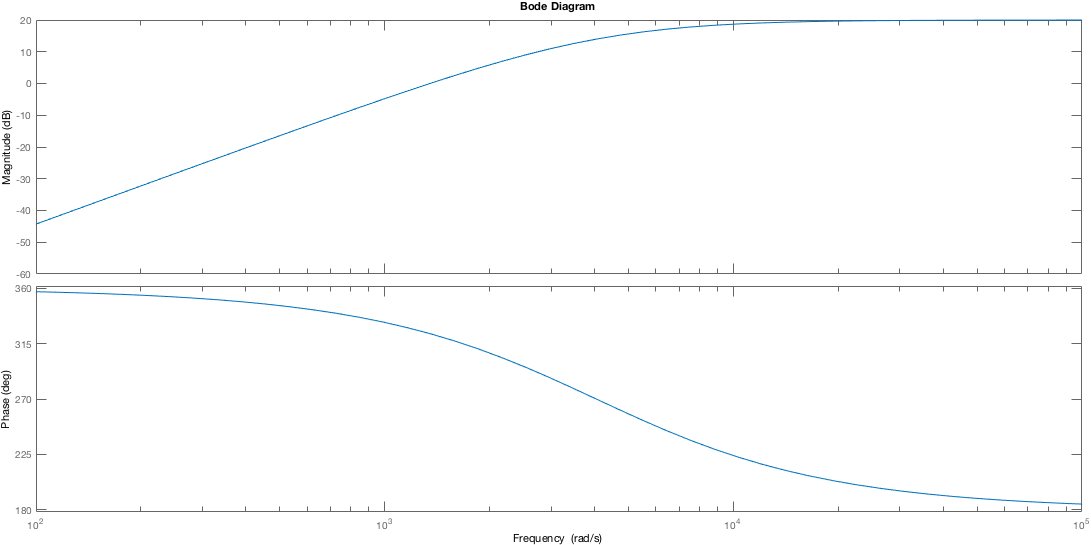
\includegraphics[scale=0.4]{q3__1.png}
			\caption{Bode plot of transfer function found in question (3b)}
		\end{figure}
		As an aside, we note that the phase response of this circuit is not what may be expected (ours starts at 0$\degree$ and ends at -180$\degree$ for increasing frequencies rather than starting at 180$\degree$ and ending at 0$\degree$). This is due to the inverting nature of our filter design as noted as the negative sign in our transfer function from (3b). \\
		However, seeing as we were designing the filter with only the magnitude response in mind, we feel that this is not an issue in answering this question.
		\\
	}
	
\end{enumerate}